\documentclass{PoS}

\usepackage{amsmath}
\usepackage{xspace}

% PROCESSES
\newcommand{\qcd}{\ensuremath{QCD}\xspace}
\newcommand{\wjets}{\ensuremath{\textrm{W+jets}}\xspace}
\newcommand{\zjets}{\ensuremath{\textrm{$Z/\gamma^*$+jets}}\xspace}
\newcommand{\vjets}{\ensuremath{\textrm{V+jets}}\xspace}
\newcommand{\ttbar}{\ensuremath{\mathrm{t}\bar{\mathrm{t}}}\xspace}
\newcommand{\tw}{\ensuremath{\mathrm{tW}}\xspace}
\newcommand{\tch}{\ensuremath{t\mathrm{\mbox{-}channel}}\xspace}


% VARIABLES
\newcommand{\pt}{\ensuremath{p_\mathrm{T}}\xspace}
\newcommand{\muiso}{\ensuremath{I_\mathrm{rel.}^{\mu}}\xspace}
\newcommand{\eiso}{\ensuremath{I_\mathrm{rel.}^{e}}\xspace}
\newcommand{\mtop}{\ensuremath{m_{\mu\nu \mathrm{b}}}\xspace}
\newcommand{\mw}{\ensuremath{m_{\mathrm{W}}}\xspace}
\newcommand{\met}{\ensuremath{{E\!\!\!/}_{\mathrm{T}}}\xspace}
\newcommand{\mtw}{\ensuremath{m_{\mathrm{T}}(\mathrm{W})}\xspace}
\newcommand{\pvmiss}{\ensuremath{\vec{p_\mathrm{T}}\hspace{-1.02em}/\kern 0.5em}\xspace}

% OTHER
\newcommand{\invfb}{\ensuremath{\mathrm{fb}^{-1}}\xspace}
\newcommand{\invpb}{\ensuremath{\mathrm{pb}^{-1}}\xspace}
\newcommand{\jprime}{\ensuremath{j^{\prime}}\xspace}
\newcommand{\qprime}{\ensuremath{q^{\prime}}\xspace}
\newcommand{\bjtop}{\ensuremath{j_\mathrm{b,top}}\xspace}


\title{Single top cross section and properties measurements in CMS}

\ShortTitle{Single top cross section and properties measurements in CMS}

\author{
    \speaker{Matthias Komm}, on behalf of the CMS collaboration\\
    Universite Catholique de Louvain (UCL) (BE)\\
    E-mail: \email{Matthias.Komm@cern.ch}
}


\abstract{TODO rephrase: At the LHC, single top quarks are predominately produced via the $t$-channel. Measuring the properties of the production process provides a crucial probe of the theory of electroweak interactions. This paper reviews recent results on cross section measurements and coupling structure studies in pp collisions by the ATLAS and CMS collaborations at center-of-mass energies of 7, 8, and 13~TeV.}

\FullConference{
    Fourth Annual Large Hadron Collider Physics\\
    13-18 June 2016\\
    Lund, Sweden
}


\begin{document}

\section{Introduction}
Measurements of single top quark production are an unique test of electroweak interactions~(EWK) involving heavy quarks. Cross section measurements of the three production modes, $t$~channel, tW~channel, and $s$~channel, offer a model-independent probe of the CKM matrix element $\mathrm{V}_\mathrm{tb}$. Furthermore, the fact that the top quark does not hadronize before its decay allows to analyse the parity-violating EWK coupling structure. In addition, one can use events containing single top quarks to probed for alternative production mechanisms as predicted in various new beyond the standard model physics~(BSM).

In this note, recent measurements of single top quark production and properties by the CMS collaboration are reviewed.


\section{Cross section measurements of $t$-channel single-top-quark production at 13~TeV}

The inclusive~(Ref.~\cite{CMS-PAS-TOP-16-003}) and differential~(Ref.~\cite{CMS-PAS-TOP-16-004}) single-top-quark cross section in $t$-channel is measured using the first pp collision data corresponding to $2.3~\mathrm{fb^{-1}}$ at a centre-of-mass energy of 13~TeV recorded in 2015. Events containing a well isolated muon with a transverse momentum of $\pt>22~\mathrm{GeV}$ and 2 or 3 jets with $\pt>40~\mathrm{GeV}$ are selected. Furthermore, multijet events are suppressed by requiring a transverse W~boson mass of $\mtw>50~\mathrm{GeV}$. A neutral network~(NN) is trained to separate the signal from the \wjets and \ttbar backgrounds. The inclusive cross section is estimated using a simultaneous binned maximum-likelihood~(ML) fit to the distribution of its discriminant~(Fig.~\ref{fig:TOP-16-003-2j1t-NN}) in signal~(2~jets, 1~b-tag) and control regions~(3~jets, 1~or 2~b-tags). The inclusive cross section is measured as $\sigma=227.8^{+33.7}_{-33.0}~\mathrm{pb}$ which agrees well with the next-to-leading order prediction of $\sigma_{t\mbox{-}\mathrm{ch.}}^\mathrm{theo.}=217.0^{+9.0}_{-7.7}~\mathrm{pb}$ using the \textsc{HATHOR}v2.1~\cite{hathor} program. Assuming $\mathrm{V}_\mathrm{td},\mathrm{V}_\mathrm{ts}\ll\mathrm{V}_\mathrm{tb} $ one finds $|\mathrm{V}_\mathrm{tb}|=\sqrt{\sigma_{t\mbox{-}\mathrm{ch.}}^\mathrm{meas.}/\sigma_{t\mbox{-}\mathrm{ch.}}^\mathrm{theo.}}=1.02\pm0.07$.


Additionally, the charge ratio is measured through separate fits to the NN distributions from top quark and antiquark events. The measured ratio is compared to the predictions by various PDF sets in Fig.~\ref{fig:TOP-16-003-2j1t-R}. A good agreement is observed.

\begin{figure}[htbp]
\begin{center}
\parbox[t]{0.49\textwidth}{\centering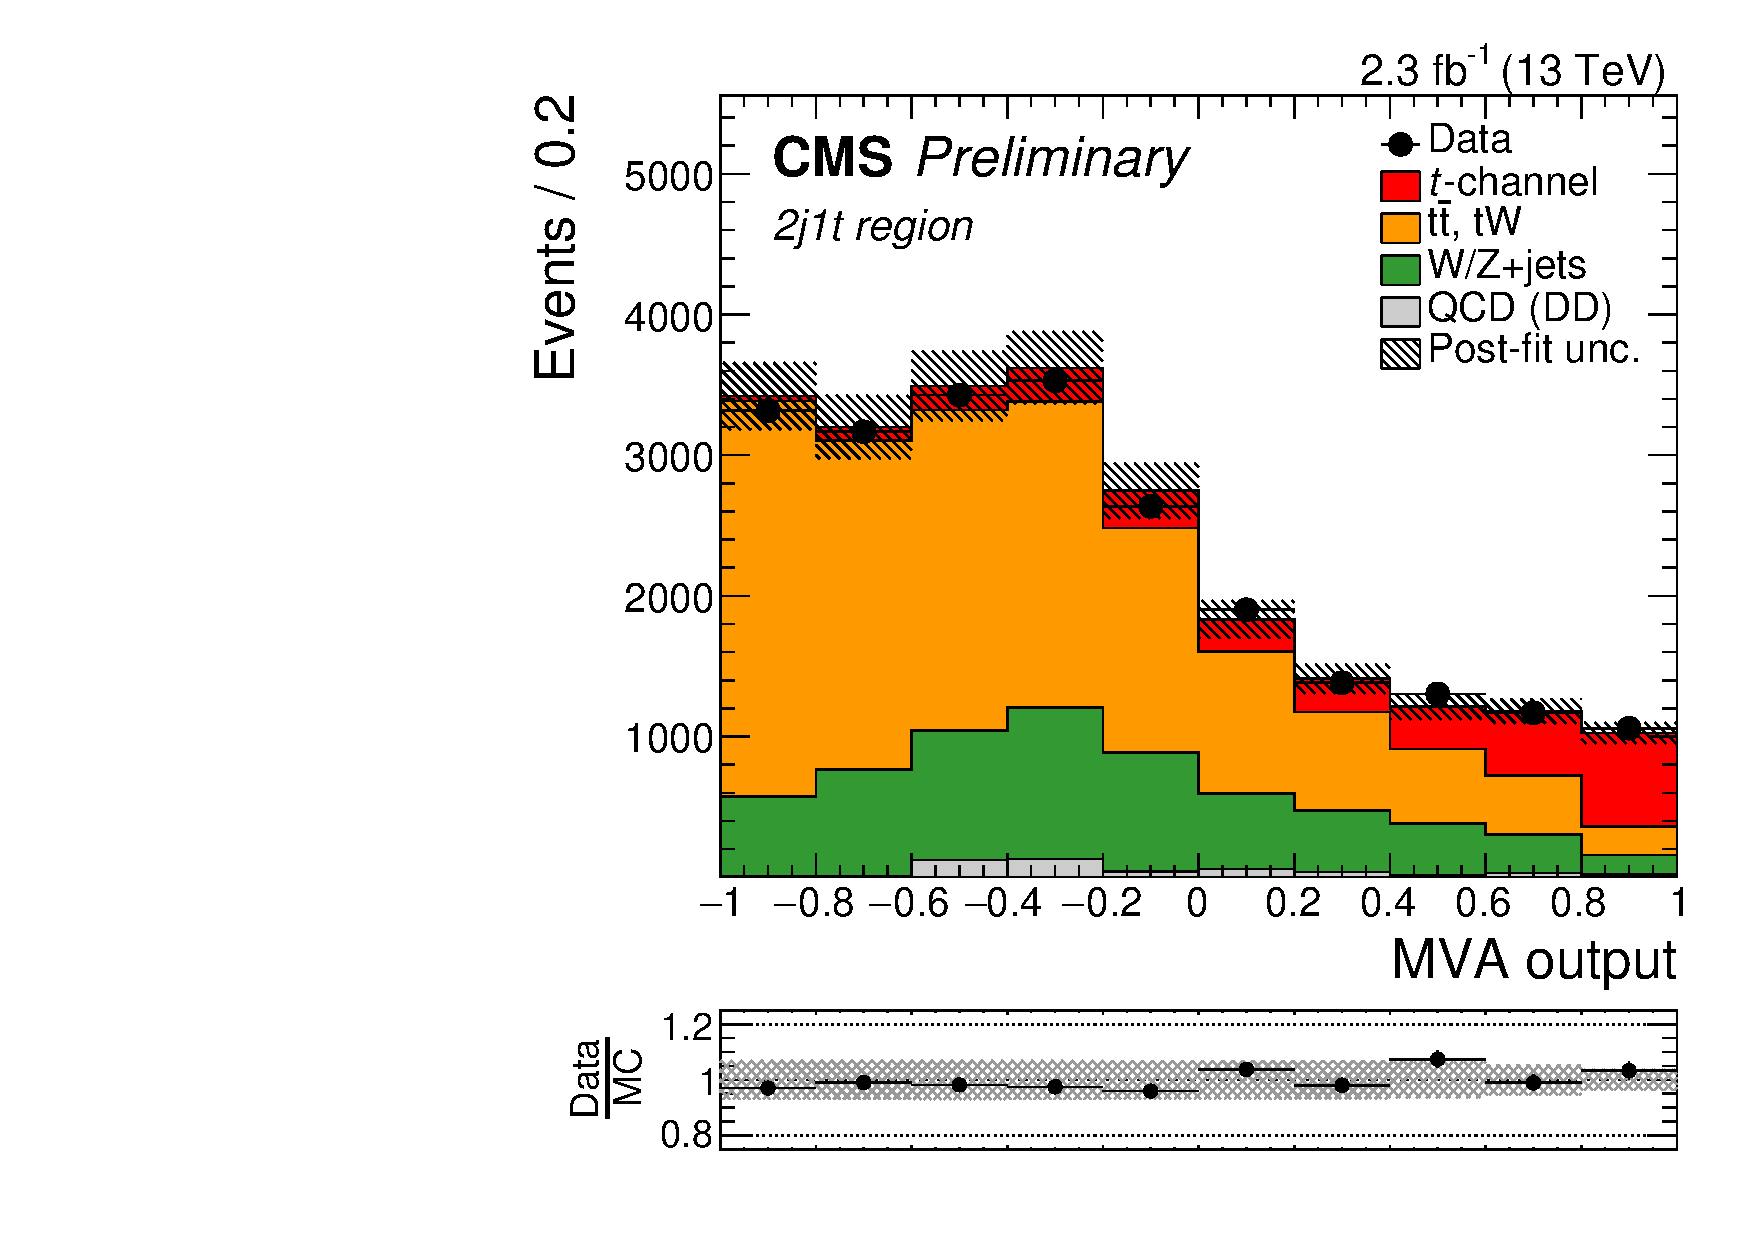
\includegraphics[width=0.4\textwidth]{figures/tchannel/2j1t_BDT.pdf}\\(a)}
\parbox[t]{0.49\textwidth}{\centering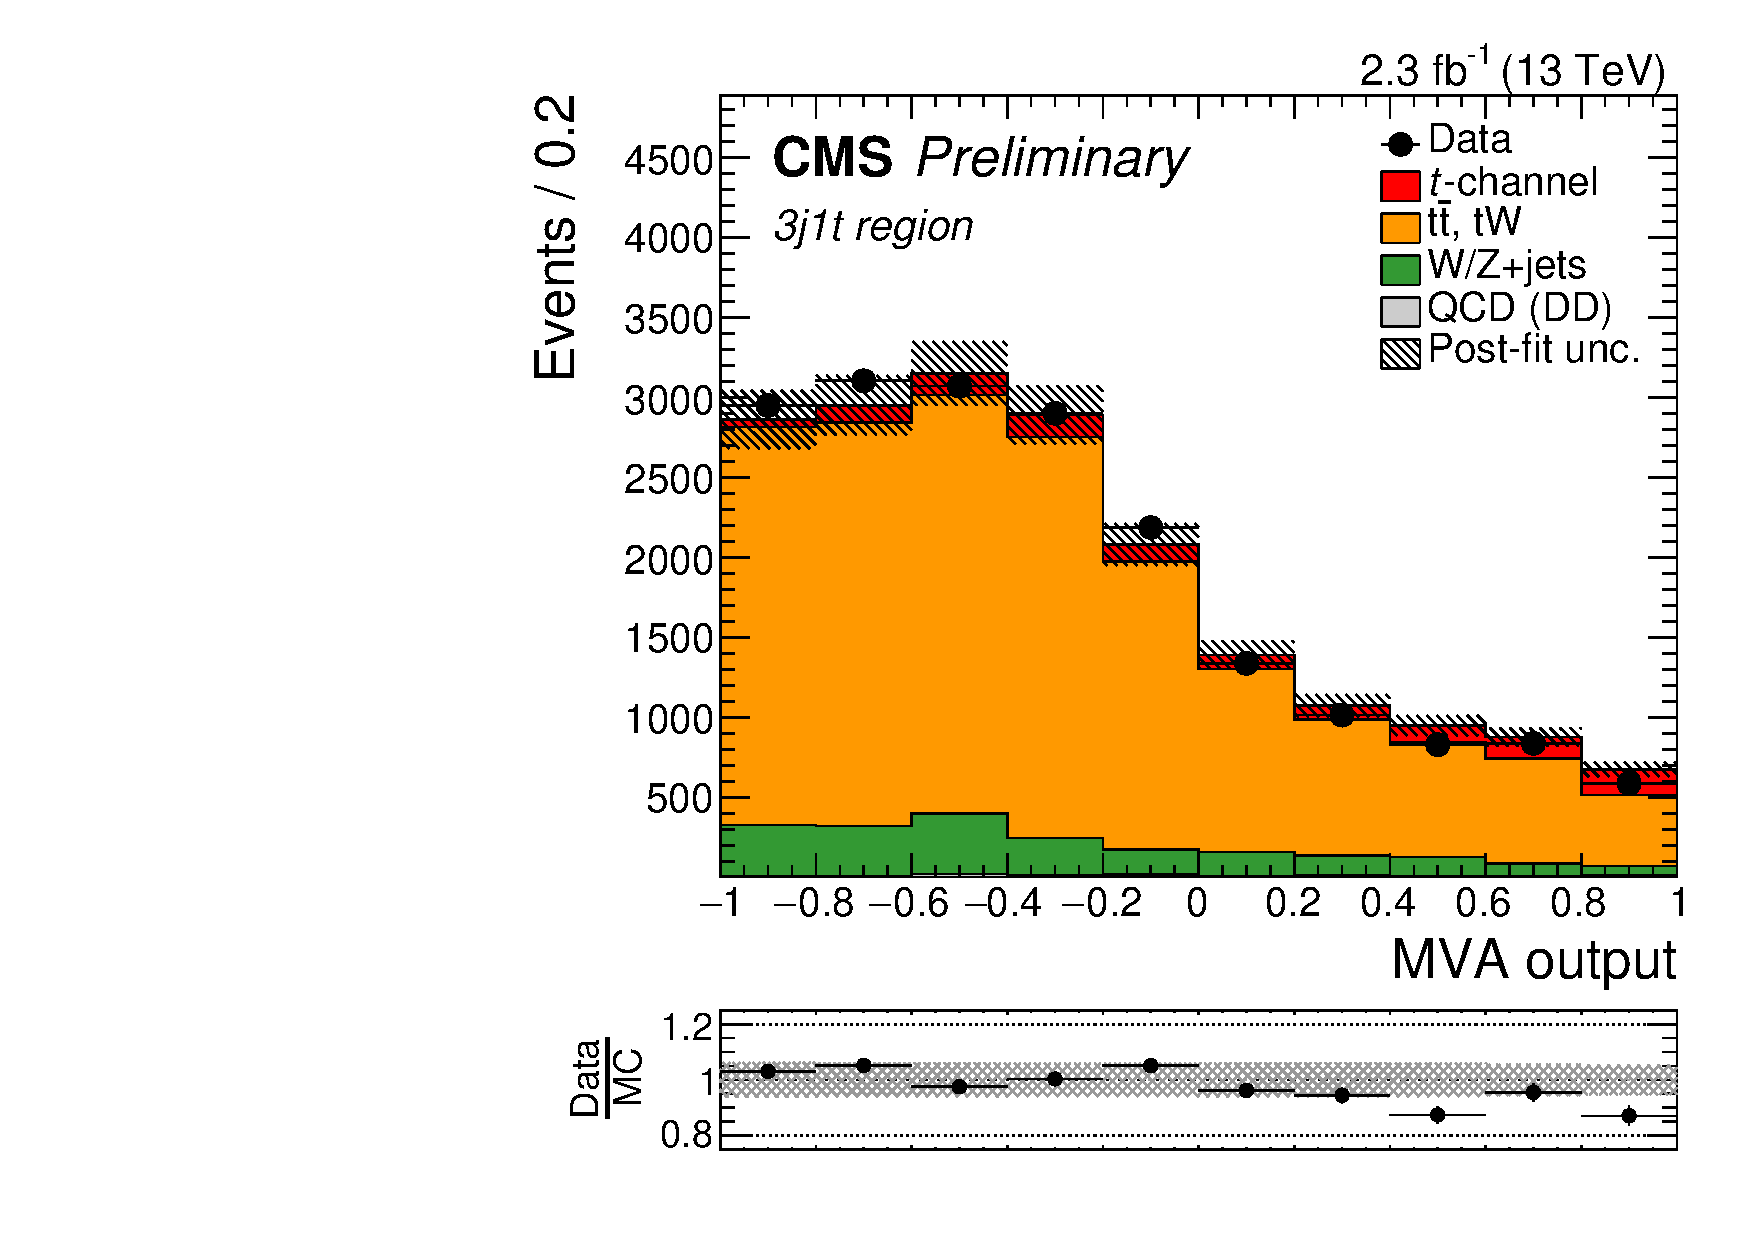
\includegraphics[width=0.4\textwidth]{figures/tchannel/3j1t_BDT.pdf}\\(b)}
\caption{\label{fig:TOP-16-003-2j1t-NN}Distributions of the neural network discriminant in the (a)~2~jets, 1~b-tag signal region and (b)~3~jets, 2~b-tags \ttbar control region. Figures are taken from Ref.~\cite{CMS-PAS-TOP-16-003}.}
\end{center}
\end{figure}



\begin{figure}[htbp]
\begin{center}
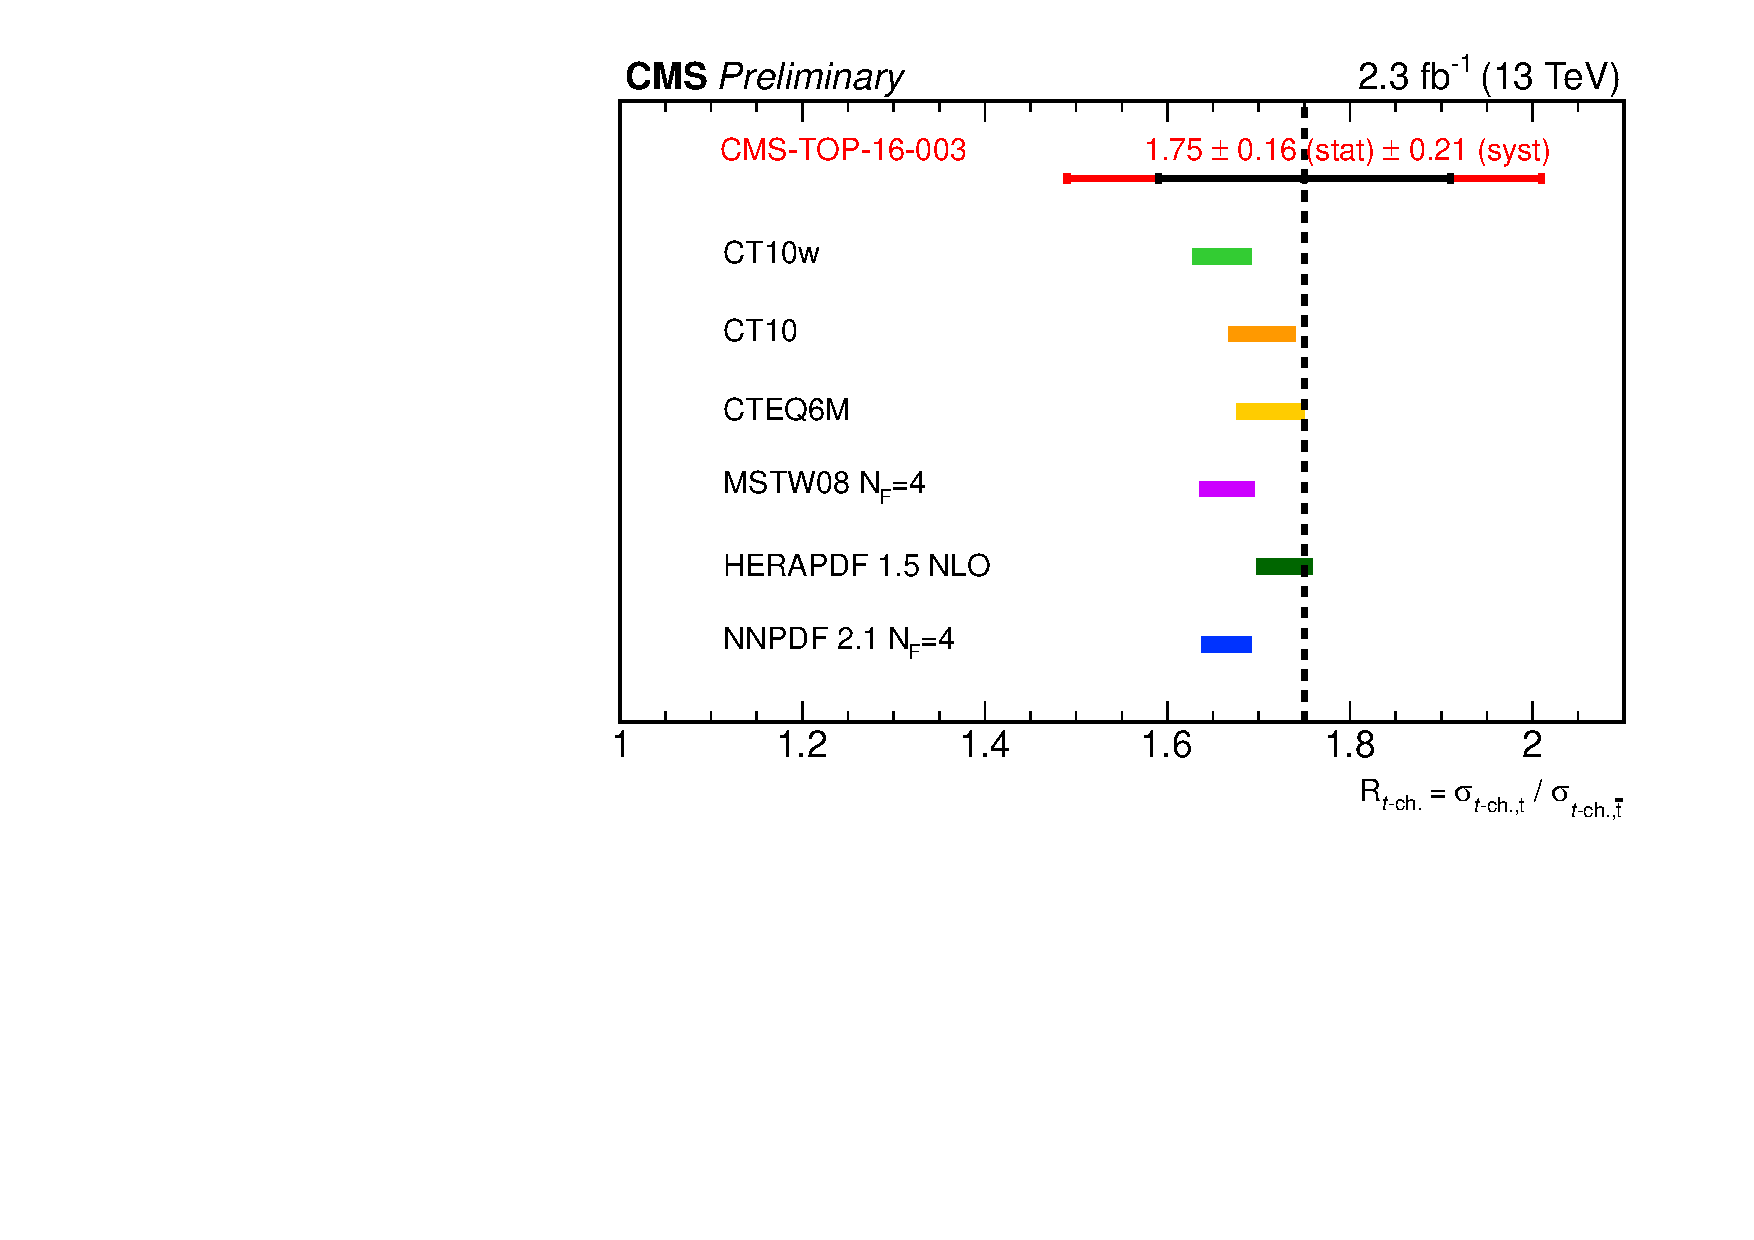
\includegraphics[width=0.7\textwidth]{figures/tchannel/ratio.pdf}
\caption{\label{fig:TOP-16-003-2j1t-R}The cross section ratio of top antiquark over top quark production compared to predictions from various PDF sets. Figure are taken from Ref.~\cite{CMS-PAS-TOP-16-003}.}
\end{center}
\end{figure}

The normalized differential cross section as a function of the top quark transverse momentum and rapidity is measured as well. For this, multiple fits are performed to the distributions of \mtw and a Boosted Decision Tree (BDT) discriminant. Each fit is restricted to events within an interval of the momentum or rapidity. The estimated signal yields are unfolded to parton level and compared to the predictions by various generators (Fig.~\ref{fig:TOP-16-004-unfolded}). No significant deviation is observed.

\begin{figure}[htbp]
\begin{center}
\parbox[t]{0.49\textwidth}{\centering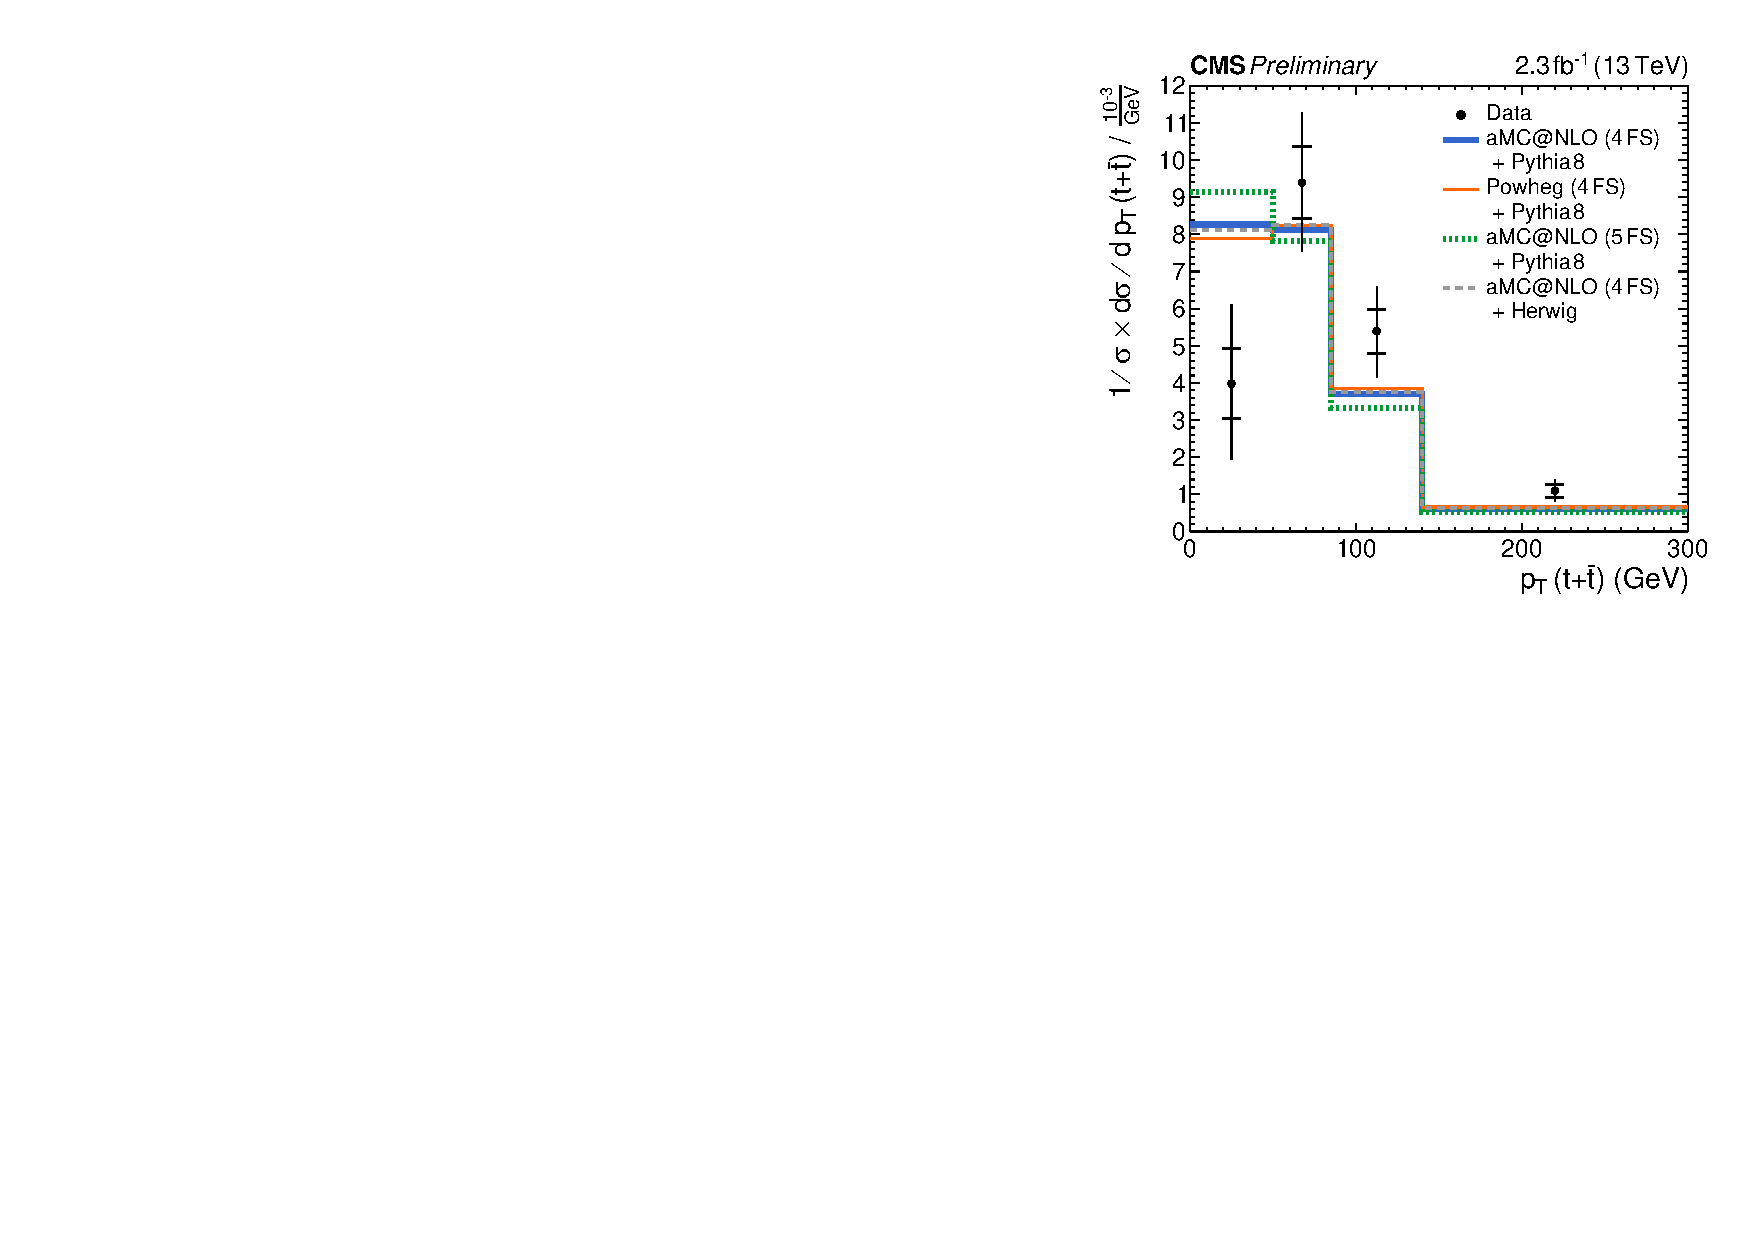
\includegraphics[width=0.42\textwidth]{figures/tchannel_diff/top_pt_unfolded.pdf}\\(a)}
\parbox[t]{0.49\textwidth}{\centering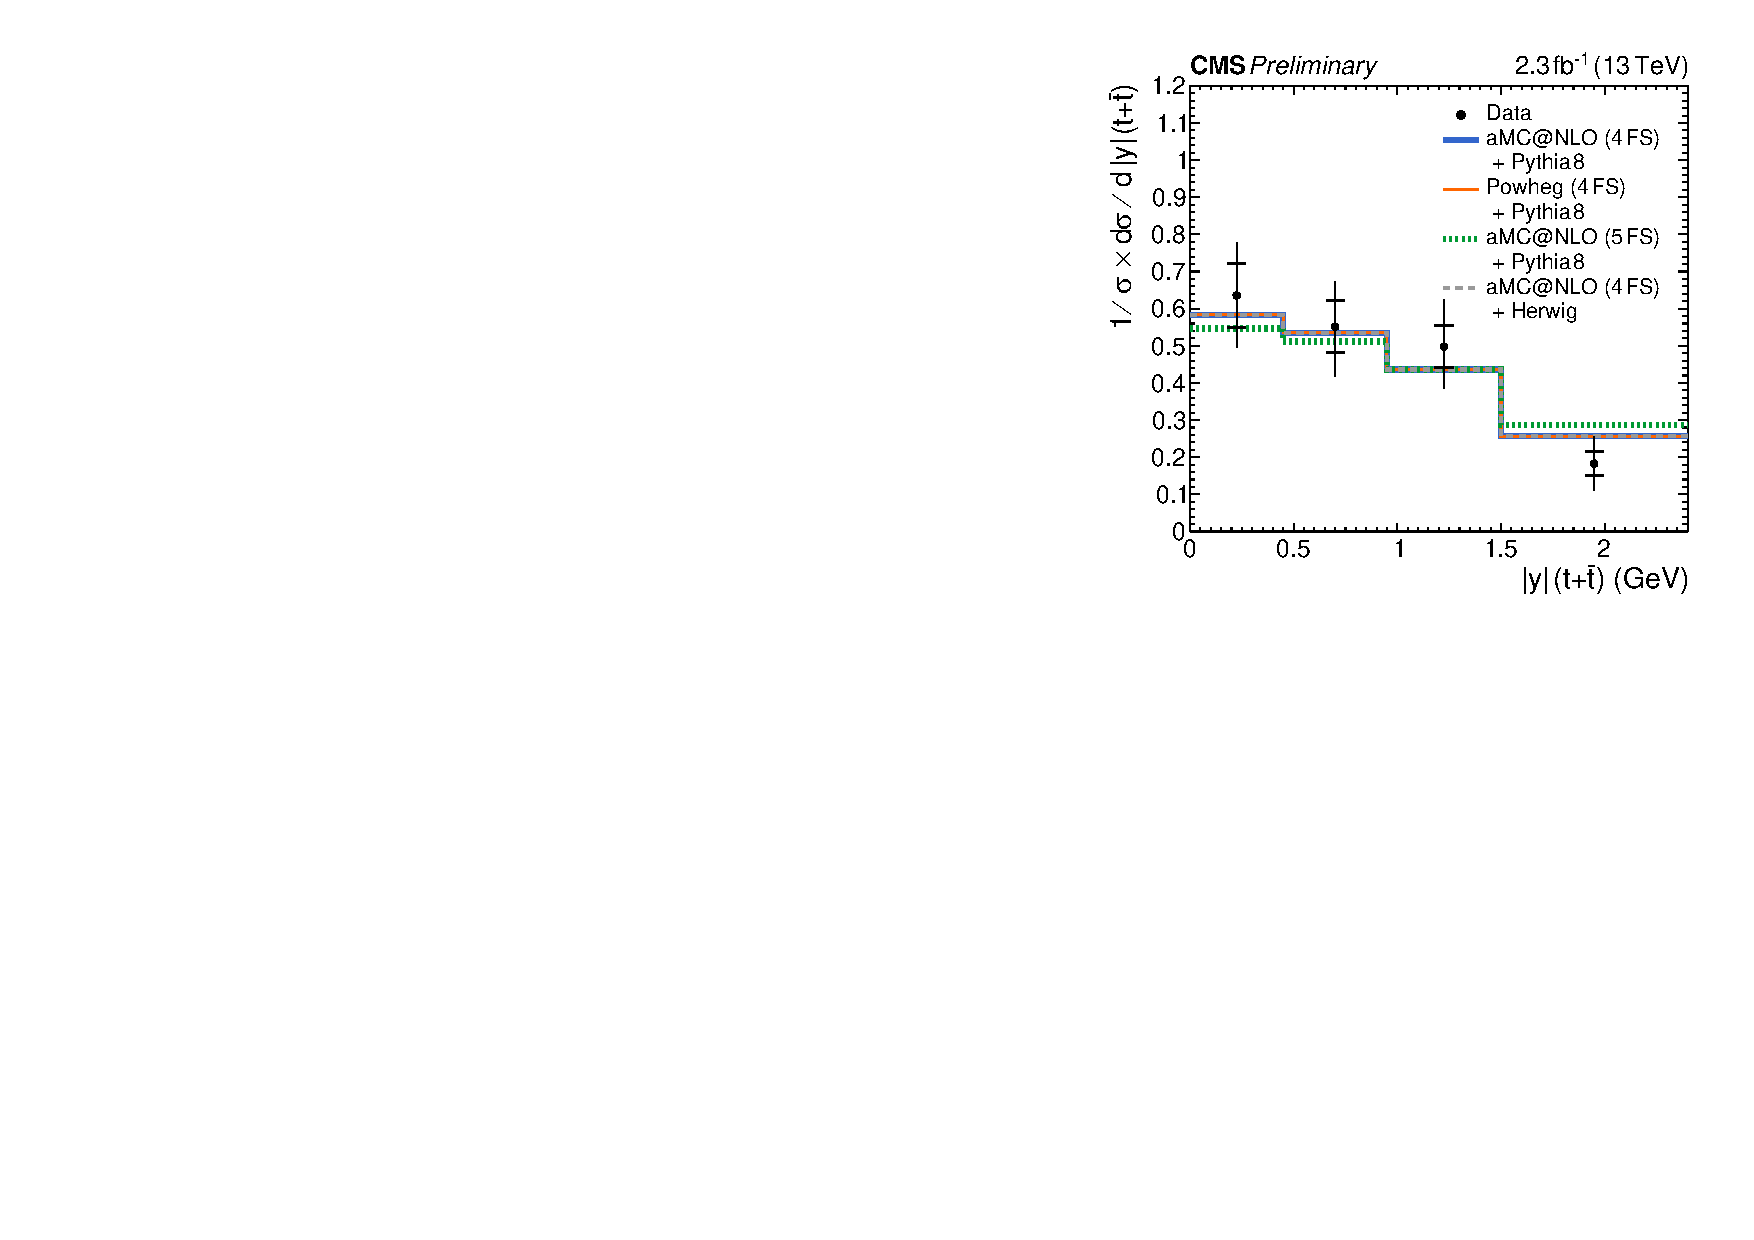
\includegraphics[width=0.42\textwidth]{figures/tchannel_diff/top_y_unfolded.pdf}\\(b)}
\caption{\label{fig:TOP-16-004-unfolded}Normalized differential cross section as a function of (a)~the top quark \pt and (b)~rapidity. Figures are taken from Ref.~\cite{CMS-PAS-TOP-16-004}.}
\end{center}
\end{figure}



\section{Search for $s$-channel single-top-quark production at 7~and 8~TeV}
At the LHC, the smallest cross section for single-top-quark production is via the $s$-channel. It is predicted to be $\sigma_{s\mbox{-}\mathrm{ch.}}^\mathrm{7~TeV}=4.6\pm0.2$ and $\sigma_{s\mbox{-}\mathrm{ch.}}^\mathrm{8~TeV}=5.6\pm0.2$ at NLO+NNLL respectively~\cite{schannel-xsec}. A new search for this production mode has been performed recently using the combined 7~and 8~TeV datasets corresponding to $5.1~\mathrm{fb}^{-1}$ and $19.7~\mathrm{fb}^{-1}$ respectively~\cite{CMS-PAS-TOP-13-009}.

Events with an isolated muon or electron with various $\pt$ thresholds ranging from $20~\mathrm{GeV}$ to $30~\mathrm{GeV}$ that follow the trigger requirements and 2 jets with $\pt>40~\mathrm{GeV}$ are selected. Multiple BDTs are trained per lepton type and centre-of-mass energy to discriminate against the overwhelming $\ttbar$ background. Figure~\ref{fig:schannel-BDT} shows the obtained distribution of the discriminats for muon events.

\begin{figure}[htbp]
\begin{center}
\parbox[t]{0.49\textwidth}{\centering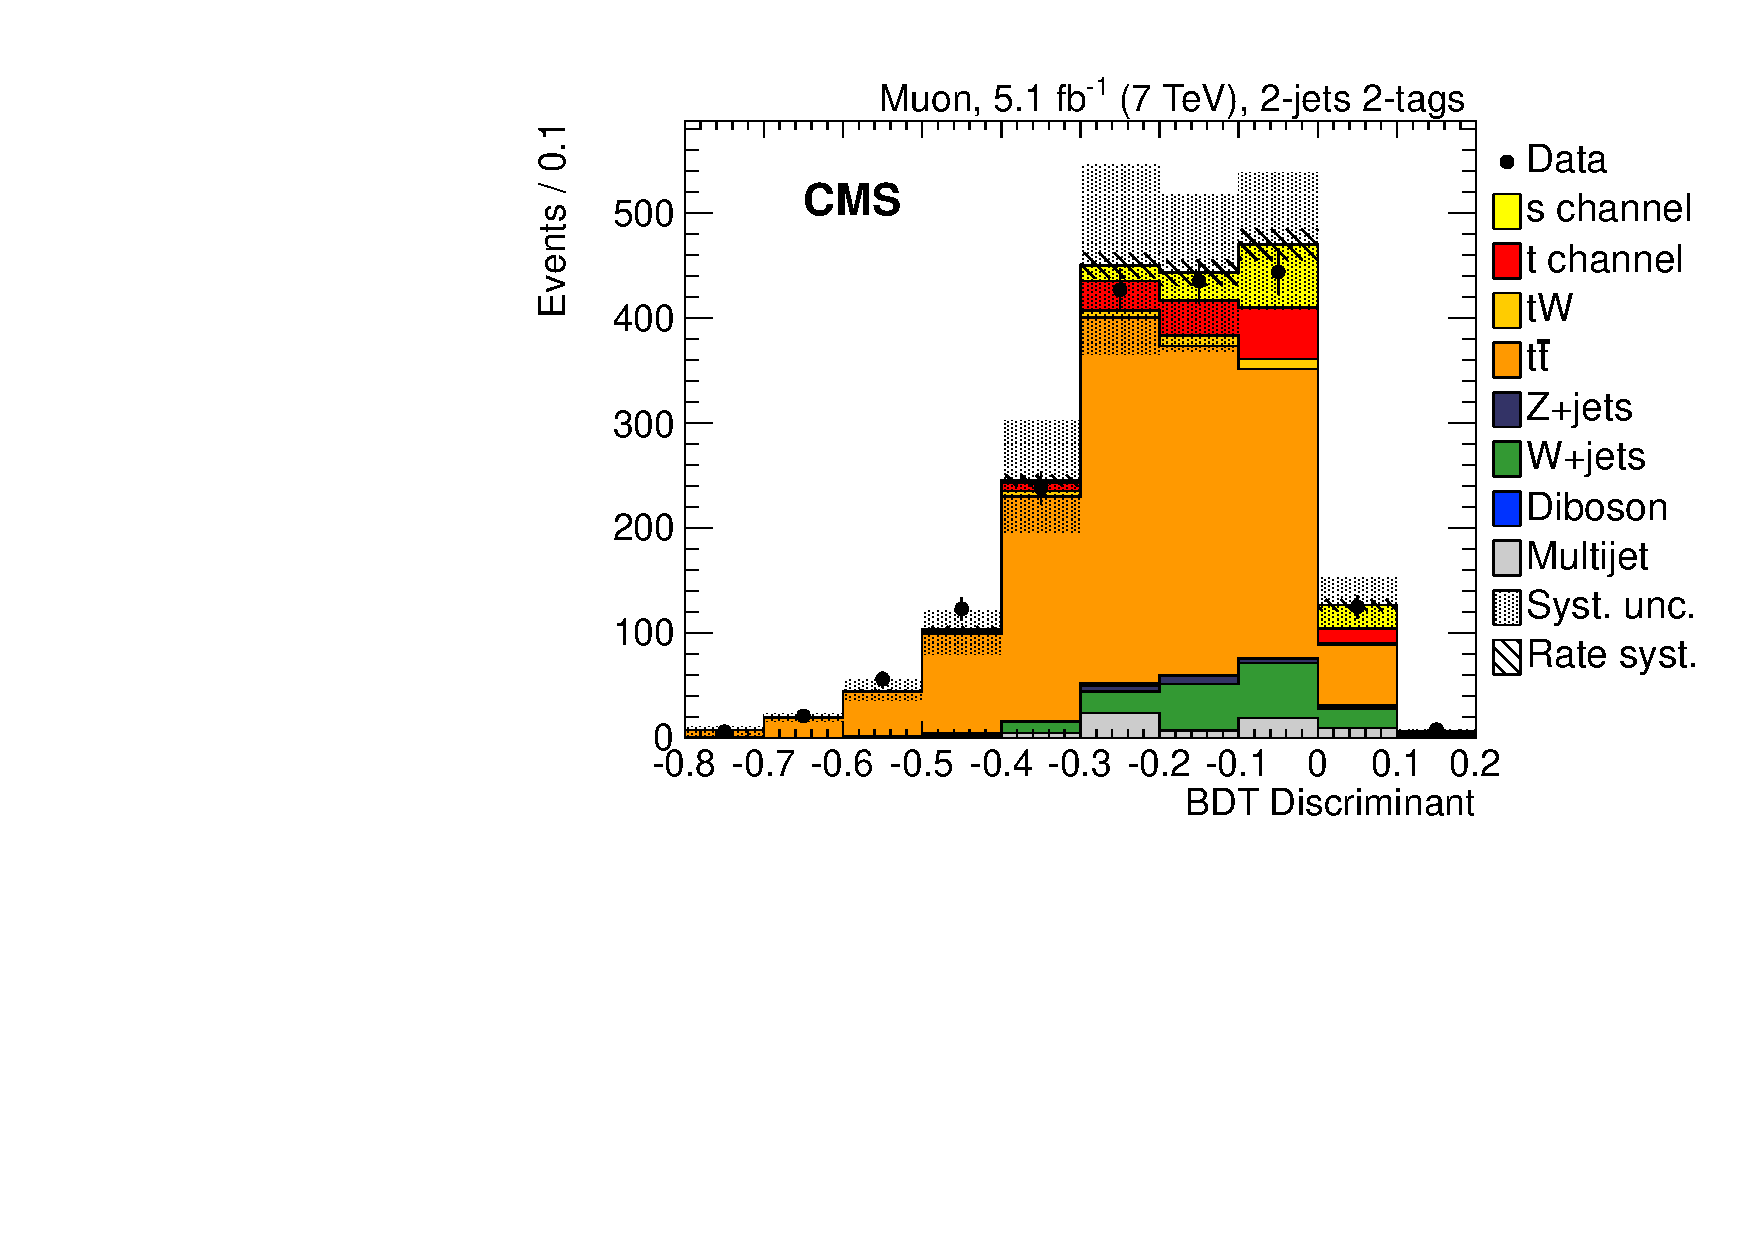
\includegraphics[width=0.48\textwidth]{figures/schannel/mu_7TeV_BDT_signal.pdf}\\(a)}
\parbox[t]{0.49\textwidth}{\centering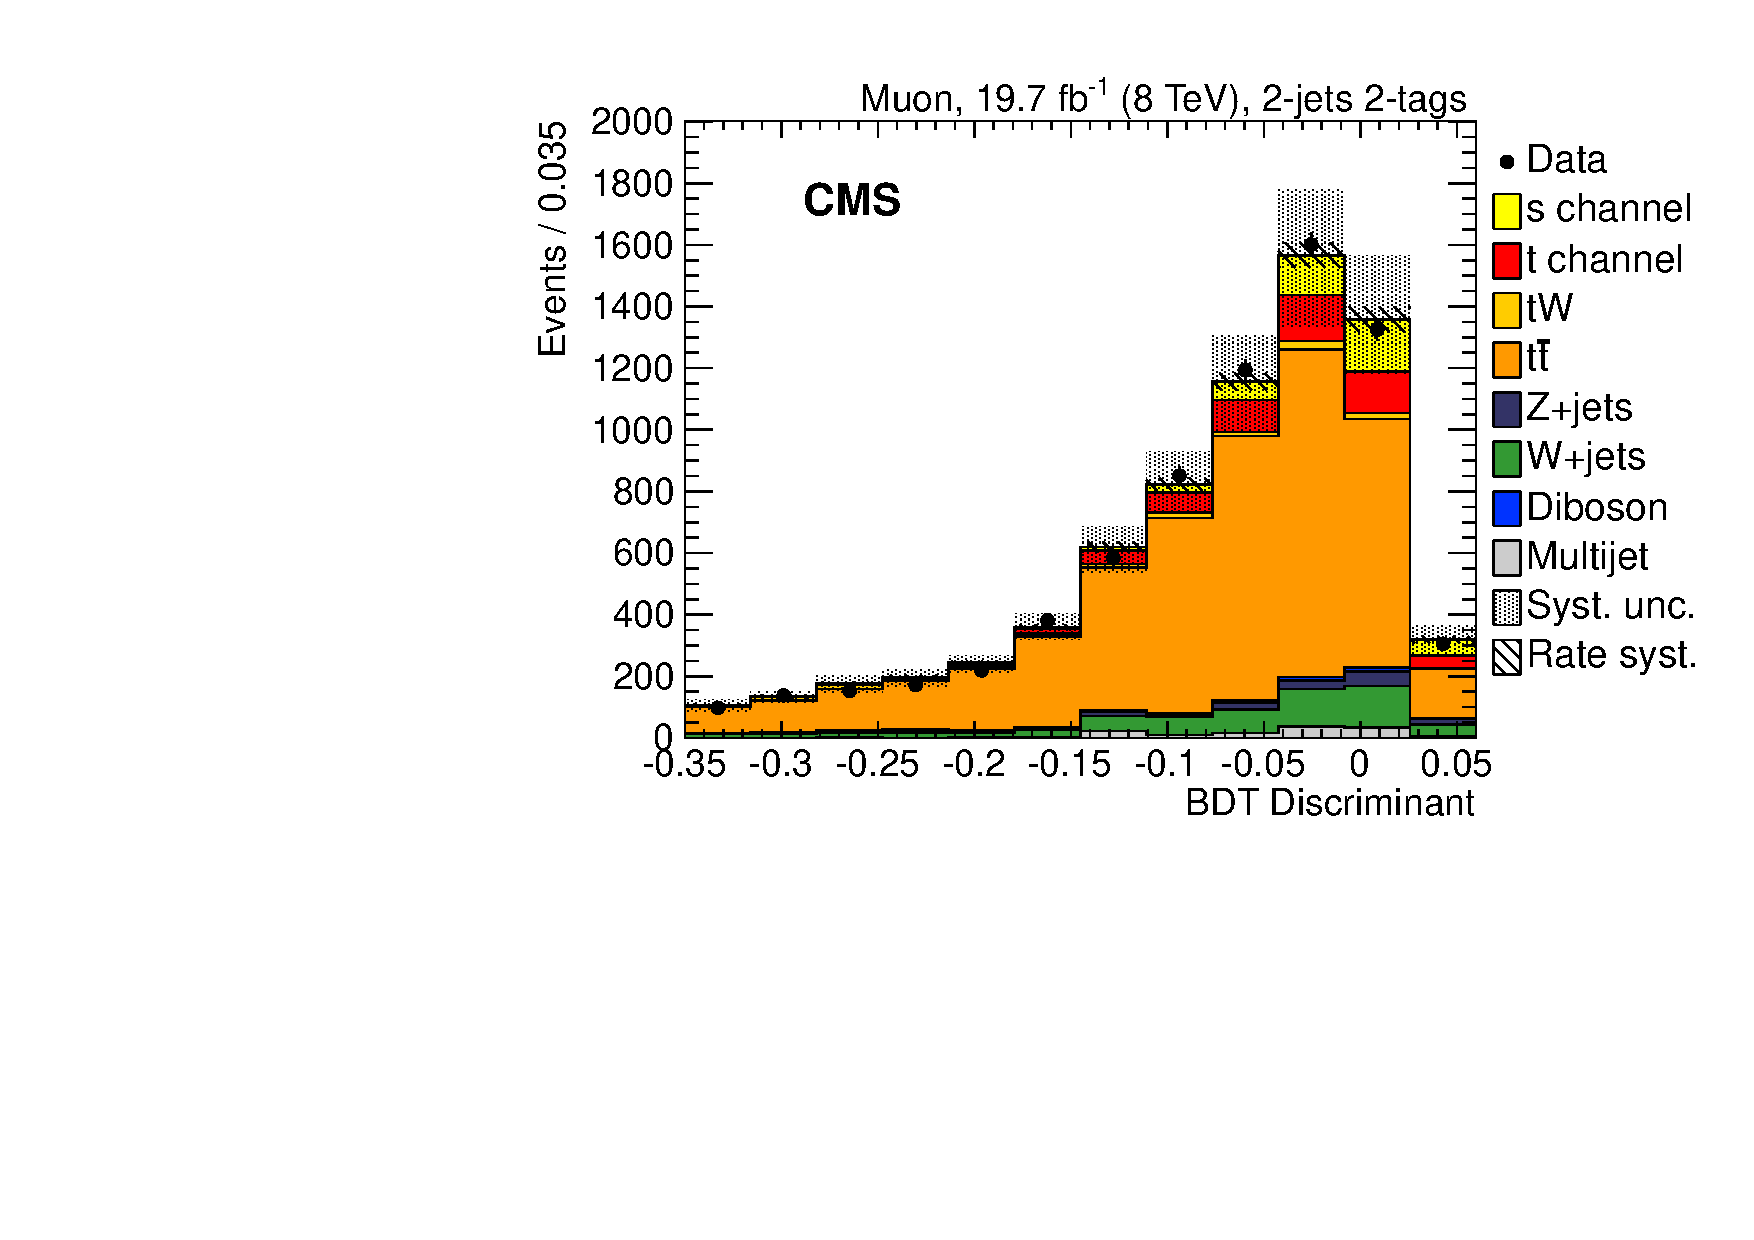
\includegraphics[width=0.48\textwidth]{figures/schannel/mu_8TeV_BDT_signal.pdf}\\(b)}
\caption{\label{fig:schannel-BDT}Distributions of the BDT discriminant in signal regions: (a)~7~TeV; (b)~8~TeV. Figures are taken from Ref.~\cite{CMS-PAS-TOP-13-009}.}
\end{center}
\end{figure}

From the distributions, the individual cross sections are estimated through ML fits as $\sigma^\mathrm{7~teV}_{s\mbox{-}\mathrm{ch.}}=7.1\pm8.1~\mathrm{pb}$ and $\sigma^\mathrm{8~teV}_{s\mbox{-}\mathrm{ch.}}=13.4\pm7.3~\mathrm{pb}$. A combined fit of the signal strength $\beta=\sigma^\mathrm{meas.}_{s\mbox{-}\mathrm{ch.}}/\sigma^\mathrm{theo.}_{s\mbox{-}\mathrm{ch.}}$ for 7~and 8~TeV yields $\beta=2.0\pm0.9$ corresponding to an observed significance of $2.5\sigma$.




\section{Measurement of $t$-channel single-top-quark polarisation}

In $t$ channel, the single top quark is expected to be produced with its spin aligned to the spectator quark because of the V-A EWK coupling structure resulting in a very high polarisation of $\mathrm{P_t}\approx1$. A closely related quantity, the top quark spin asymmetry as suggested in Ref.~\cite{wbeyond} has been measured using the 8~TeV dataset~\cite{CMS-PAS-TOP-13-001}. It is defined as 

\begin{equation}
A=\frac{N(\cos\theta^{\star}>0)-N(\cos\theta^{\star}<0)}{N(\cos\theta^{\star}>0)+N(\cos\theta^{\star}<0)}=\frac{1}{2}\alpha_{l}\mathrm{P_{t}}
\end{equation}

where the angle, $\cos\theta^{\star}$, is taken between the lepton from the top quark decay and the spectator quark in the top quark rest frame. The spin-analyzing power is denoted as $\alpha_{l}$.

To measure the asymmetry, events containing an isolated muon with $\pt>26~\mathrm{GeV}$ and 2 or 3 jets with $\pt>40~\mathrm{GeV}$ are selected. Multijet events are rejected by applying an additional selection on a dedicated BDT discriminator value. A second BDT is used to select data in a signal-enhanced phase space. After estimating the overall normalizations of the signal and background processes, the reconstructed $\cos\theta^{\star}$ distribution is unfolded to parton level. Figure~\ref{fig:costheta} shows the distributions before and after unfolding. An overall trend in the ratio between data and the predictions by various MC generators is observed.

\begin{figure}[htbp]
\begin{center}
\parbox[t]{0.55\textwidth}{\centering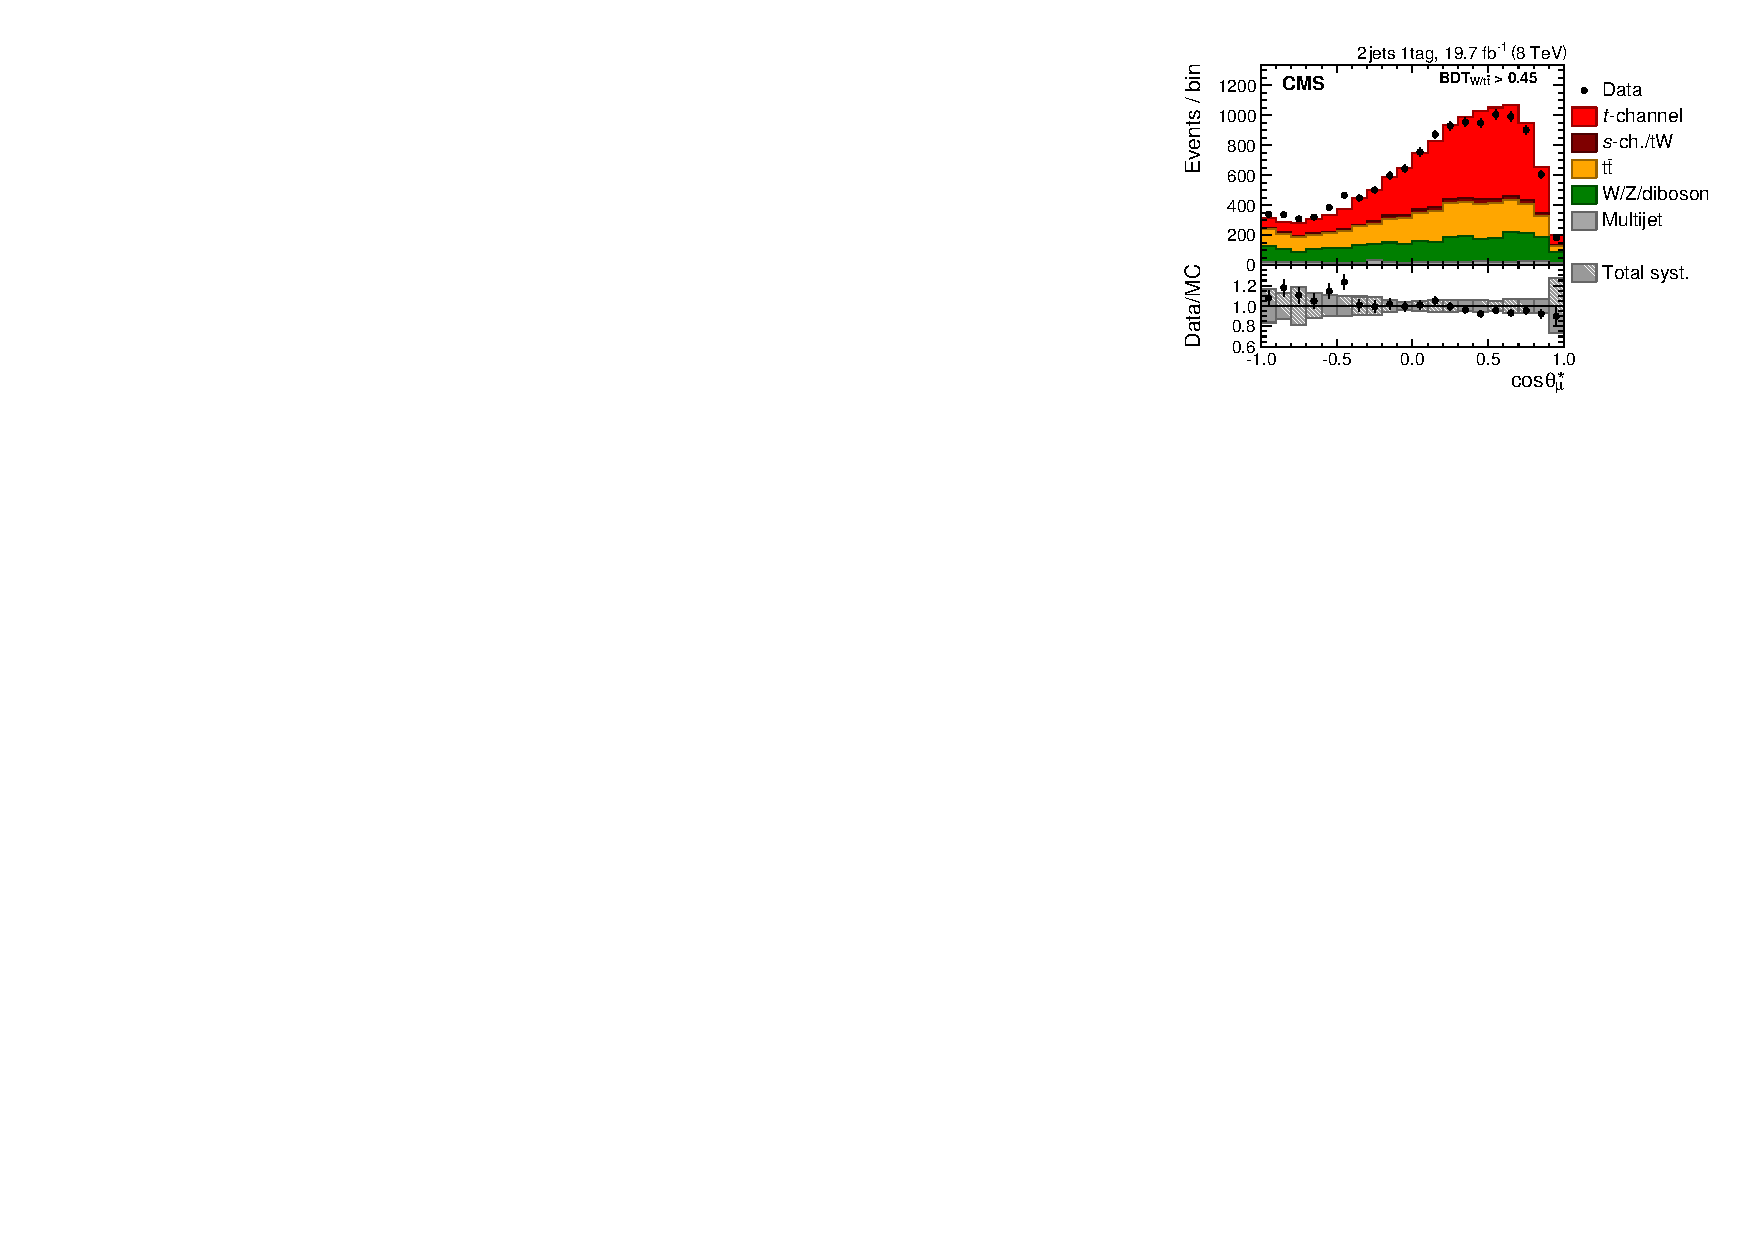
\includegraphics[width=0.54\textwidth]{figures/polarization/2j1t_cos_theta.pdf}\\(a)}
\parbox[t]{0.44\textwidth}{\centering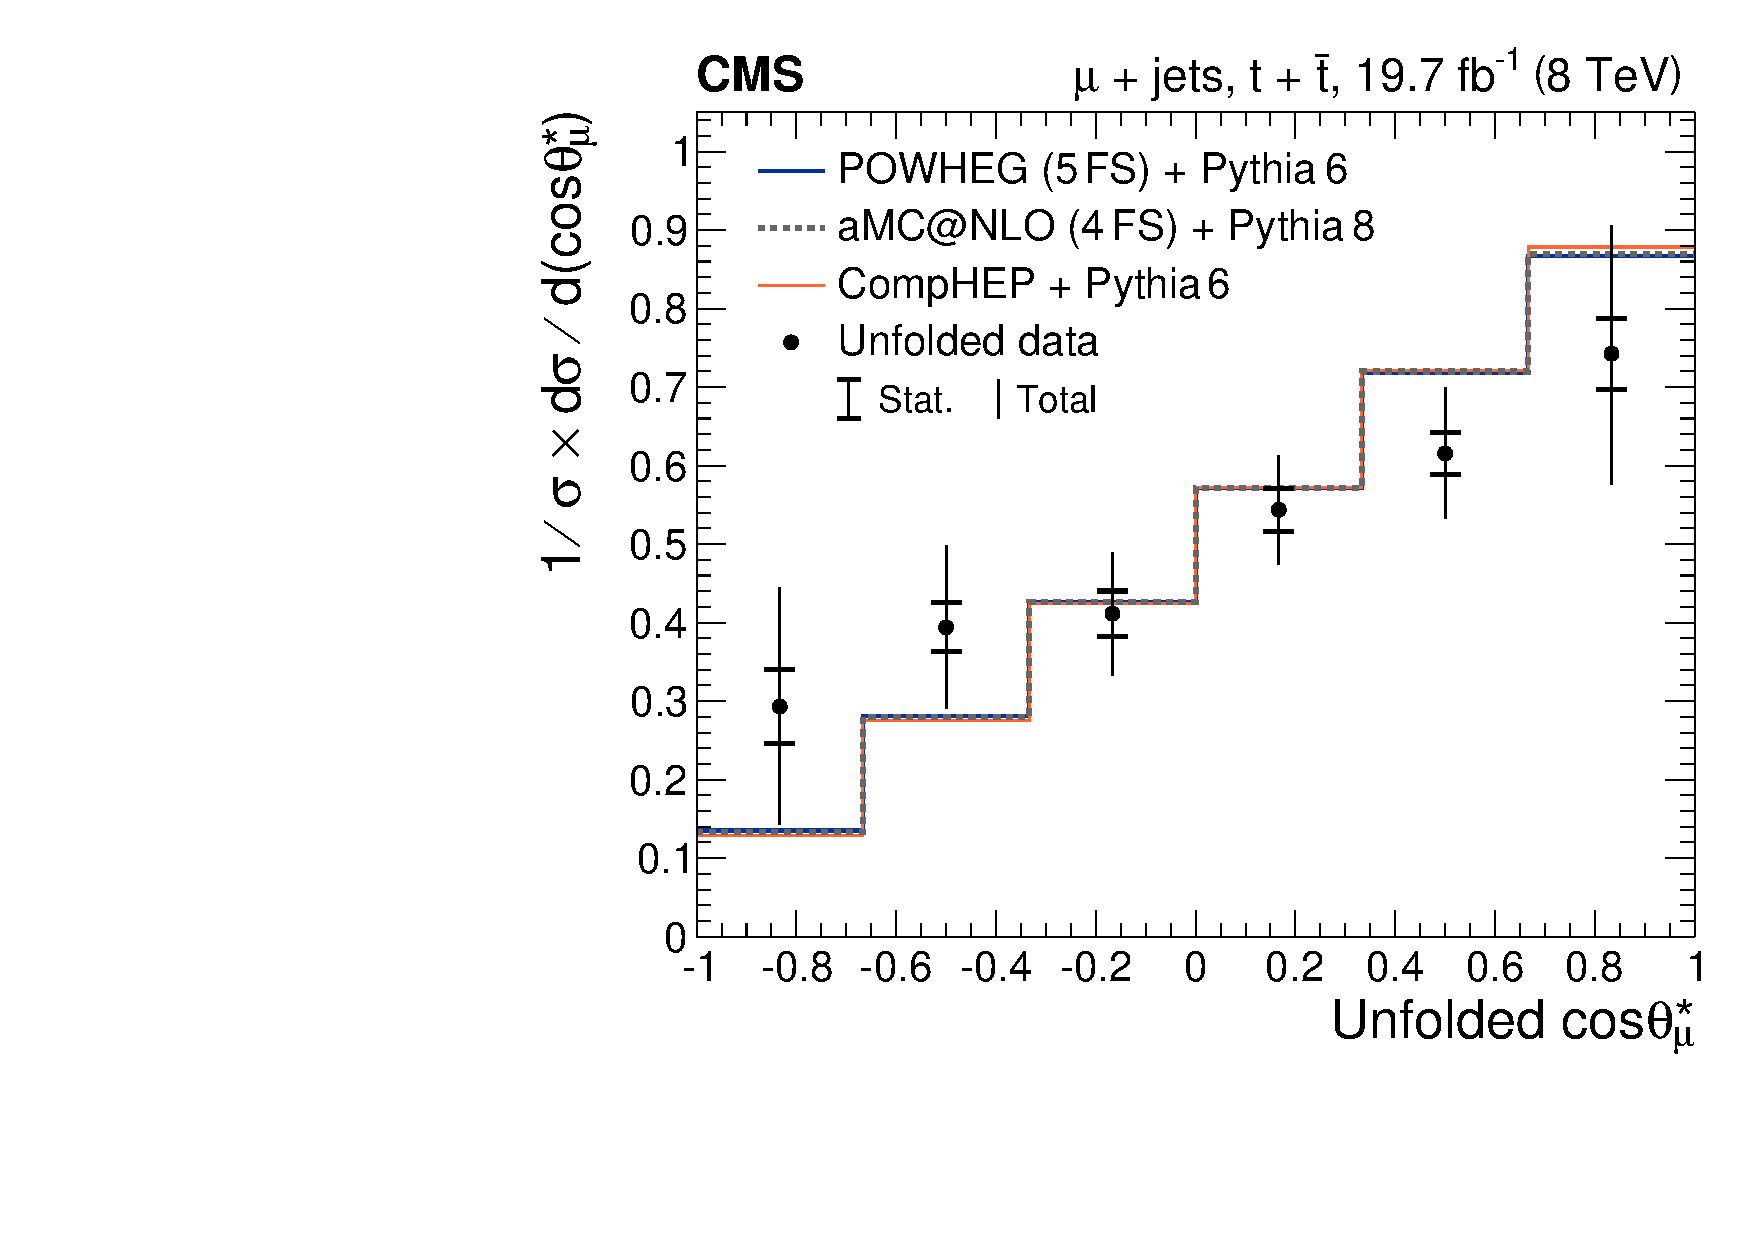
\includegraphics[width=0.43\textwidth]{figures/polarization/cos_theta_unfolded.pdf}\\(b)}
\caption{\label{fig:costheta}Distributions of the (a)~reconstructed and (b)~unfolded polarisation angle. Figures are taken from Ref.~\cite{CMS-PAS-TOP-13-001}.}
\end{center}
\end{figure}

The top quark spin asymmetry is measured as $A=0.26\pm0.11$ which is compatible with the SM expectation of $A=0.44$ within 2.0~standard deviations.


\section{Search for flavour changing interactions between top-quarks and photons}

In the SM, flavor changing neutral currents~(FCNC) are heavily suppressed by the GIM mechanism~\cite{fcnc}. An enhancement of such interactions can be characterized through an effective extensions of the SM by introducing new operators with the couplings stengths $\kappa_{\mathrm{tu}\gamma}/\Lambda$ and $\kappa_{\mathrm{tc}\gamma}/\Lambda$ leading to direct $\mathrm{t}\to\mathrm{u}\gamma$ and $\mathrm{t}\to\mathrm{c}\gamma$ decays of the top quark, respectively~\cite{minimal-anom-set}. 


A search for such FCNC couplings in the single top quark sector has been performed using the 8~TeV dataset~\cite{CMS-PAS-TOP-14-003}. Selected events contain the signature of a decayed single top quark consisting of an isolated muon with $\pt>26~\mathrm{GeV}$, a b-tagged jet with $\pt>30~\mathrm{GeV}$, and missing transverse energy $\mathrm{E}^\mathrm{miss}_\mathrm{T}>30~\mathrm{GeV}$. Additionally, the presence of an isolated photon with $\pt>50~\mathrm{GeV}$ is required that would recoil against the top quark due to the FCNC coupling.


Two BDTs are trained to separate the remaining backgrounds from either the $\mathrm{t}\to\mathrm{u}\gamma$ or the $\mathrm{t}\to\mathrm{c}\gamma$ signal. The resulting distributions of their discriminants are shown in Fig.~\ref{fig:FCNC}. The shapes and normalizations of the $\mathrm{W}\mbox{+}\mathrm{jets}$, $\mathrm{W}\gamma\mbox{+}\mathrm{jets}$ backgrounds have been estimated from data in a sideband region. No excess of data hinting torwards FCNC coulings is observed. Therefore, upper limits are set on the coupling strengths. The limits are shown in Figure~\ref{fig:FCNClimit} together with the results from other measurements.


\begin{figure}[htbp]
\begin{center}
\parbox[t]{0.49\textwidth}{\centering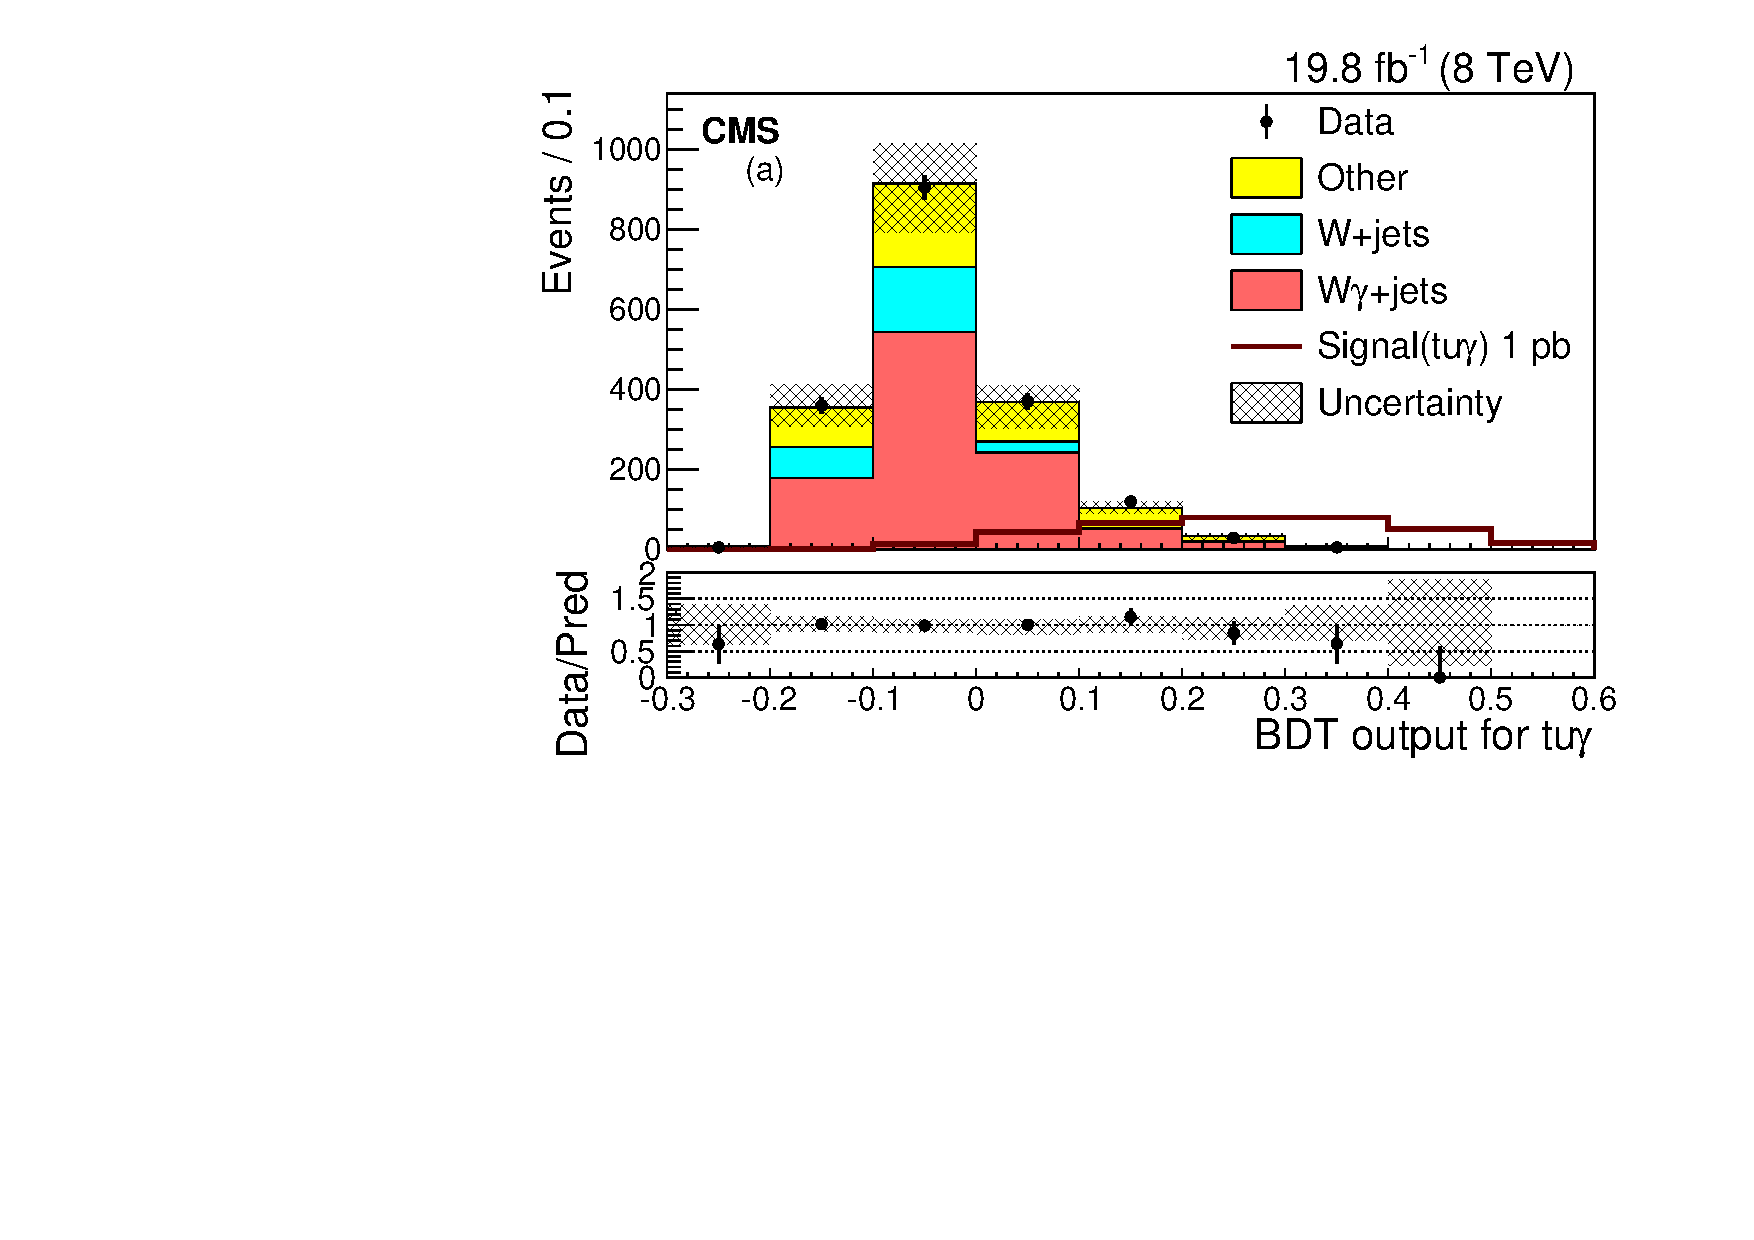
\includegraphics[width=0.48\textwidth]{figures/FCNC/BDT_utg.pdf}\\(a)}
\parbox[t]{0.49\textwidth}{\centering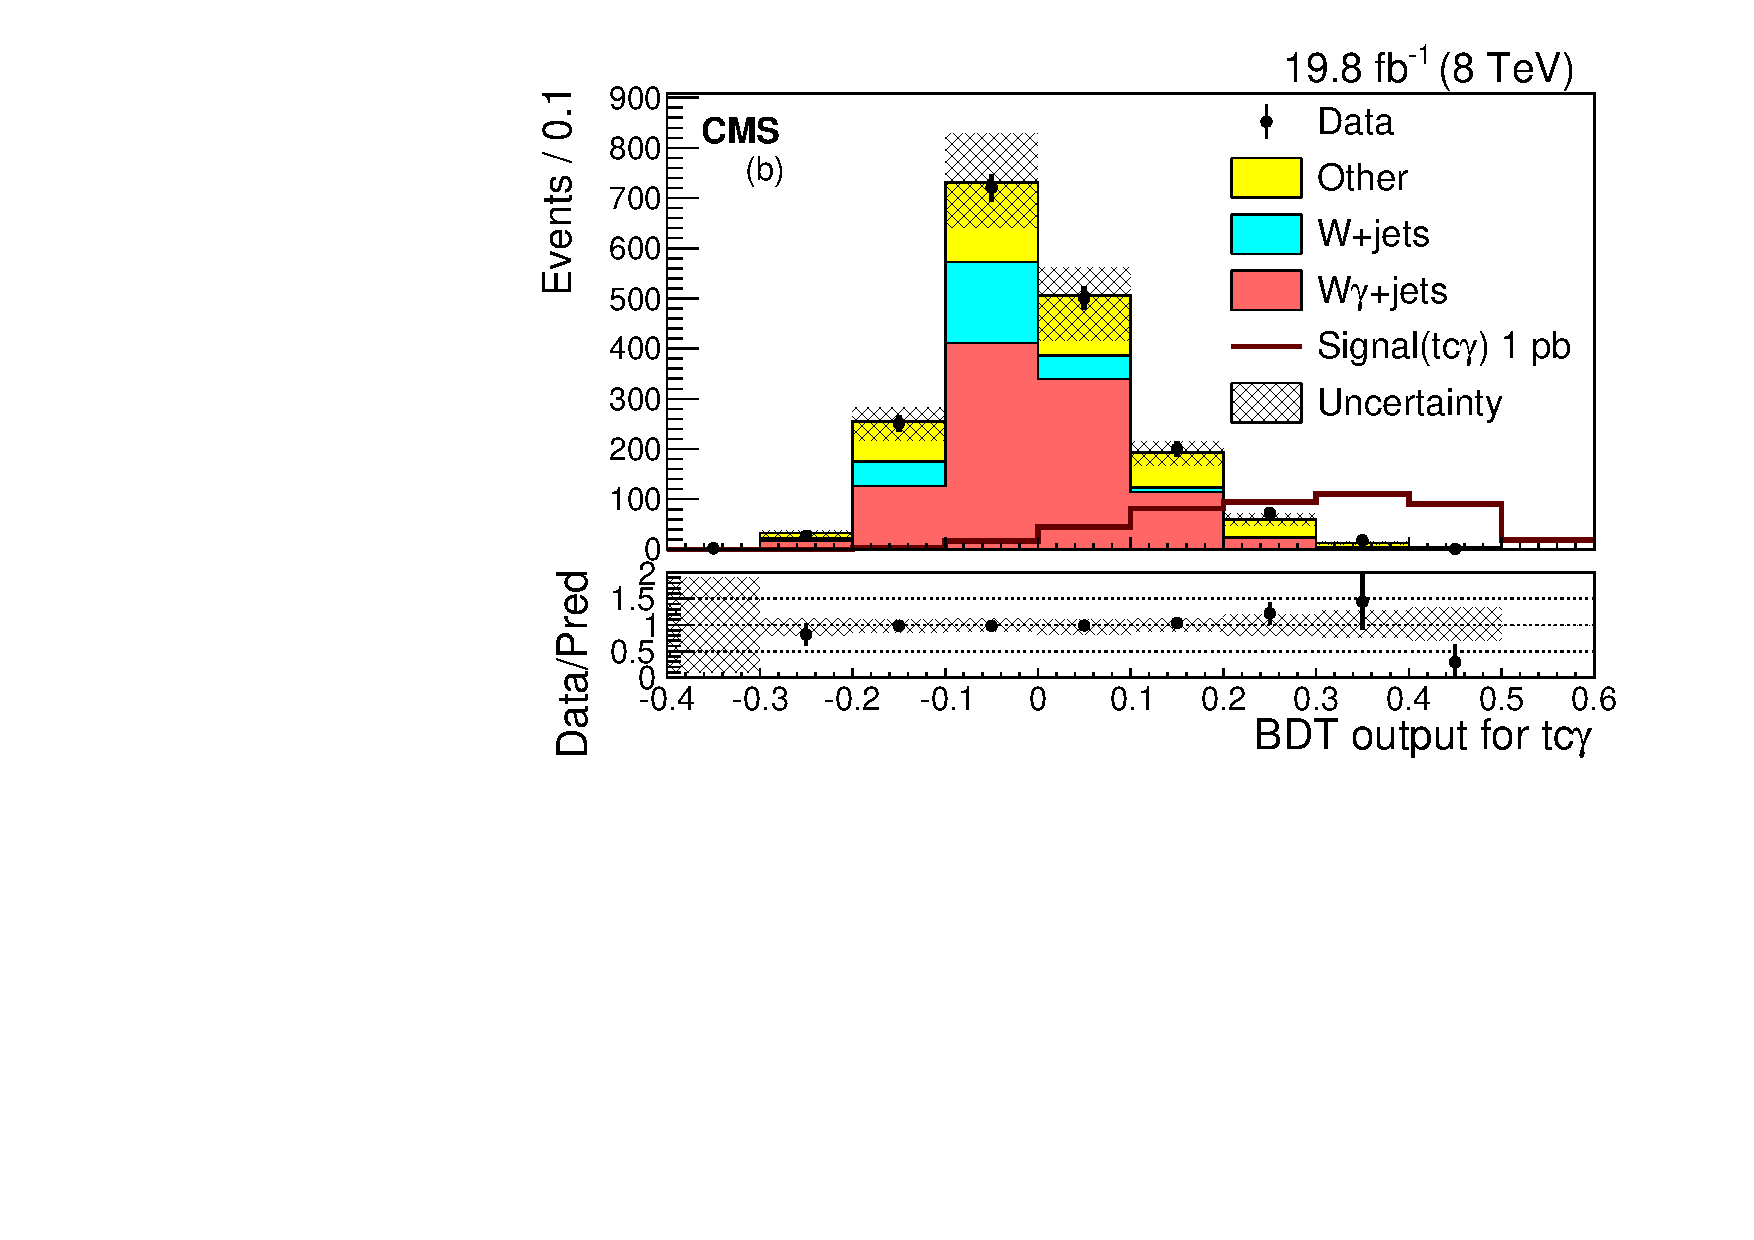
\includegraphics[width=0.48\textwidth]{figures/FCNC/BDT_ctg.pdf}\\(b)}
\caption{\label{fig:FCNC}Distributions of the FCNC BDT discriminants: (a)~$\mathrm{tu}\gamma$-, (b)~$\mathrm{tc}\gamma$-vertex. Figures are taken from Ref.~\cite{CMS-PAS-TOP-14-003}.}
\end{center}
\end{figure}


\begin{figure}[htbp]
\begin{center}
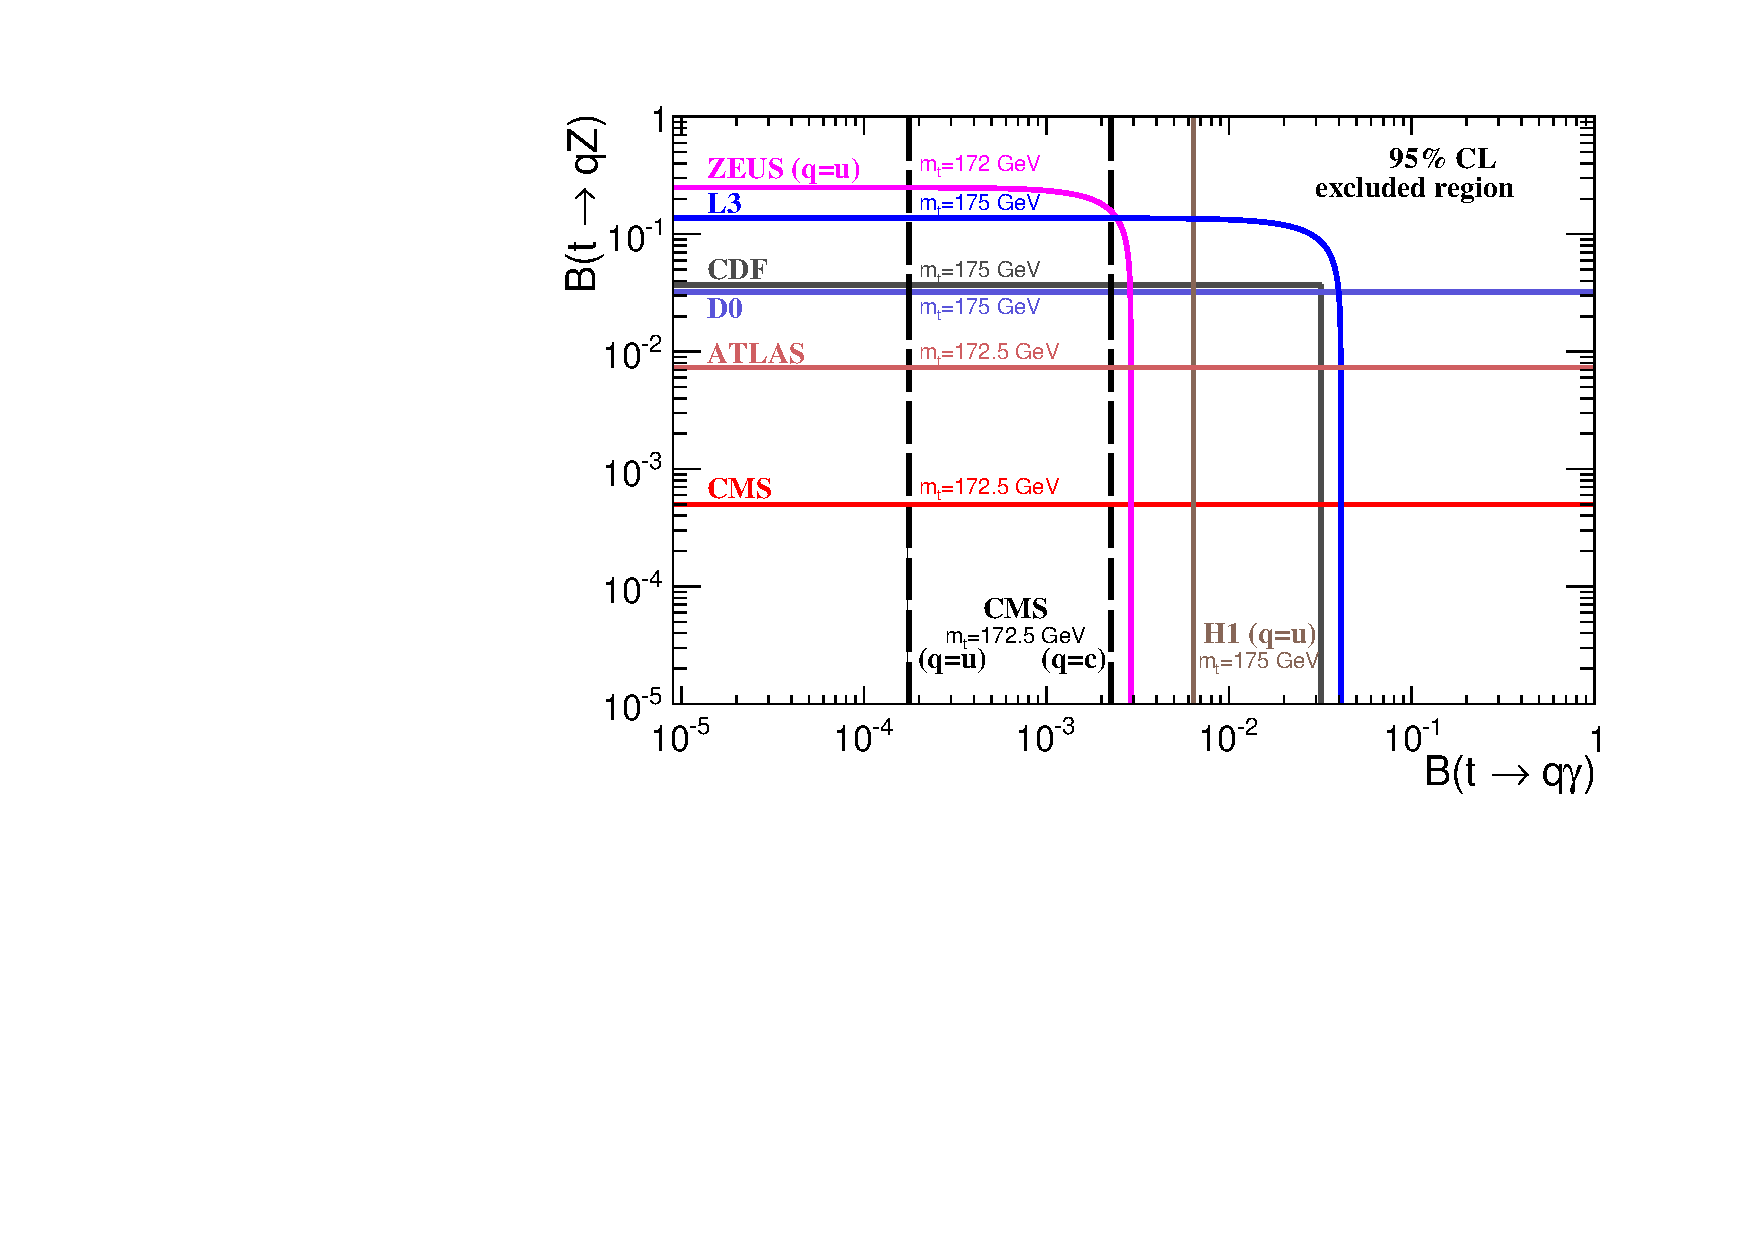
\includegraphics[width=0.7\textwidth]{figures/limits.pdf}
\caption{\label{fig:FCNClimit}Overview of limits on FCNC $\mathrm{t}\to\mathrm{q}\gamma$ and $\mathrm{t}\to\mathrm{qZ}$ branching ratios from various experimemts. Figure is taken from Ref.~\cite{CMS-PAS-TOP-14-003}.}
\end{center}
\end{figure}



\section{Conclusion}

Recent measurements and searches using single top quarks by the CMS collaboration have been presented. 

\begin{figure}[htbp]
\begin{center}
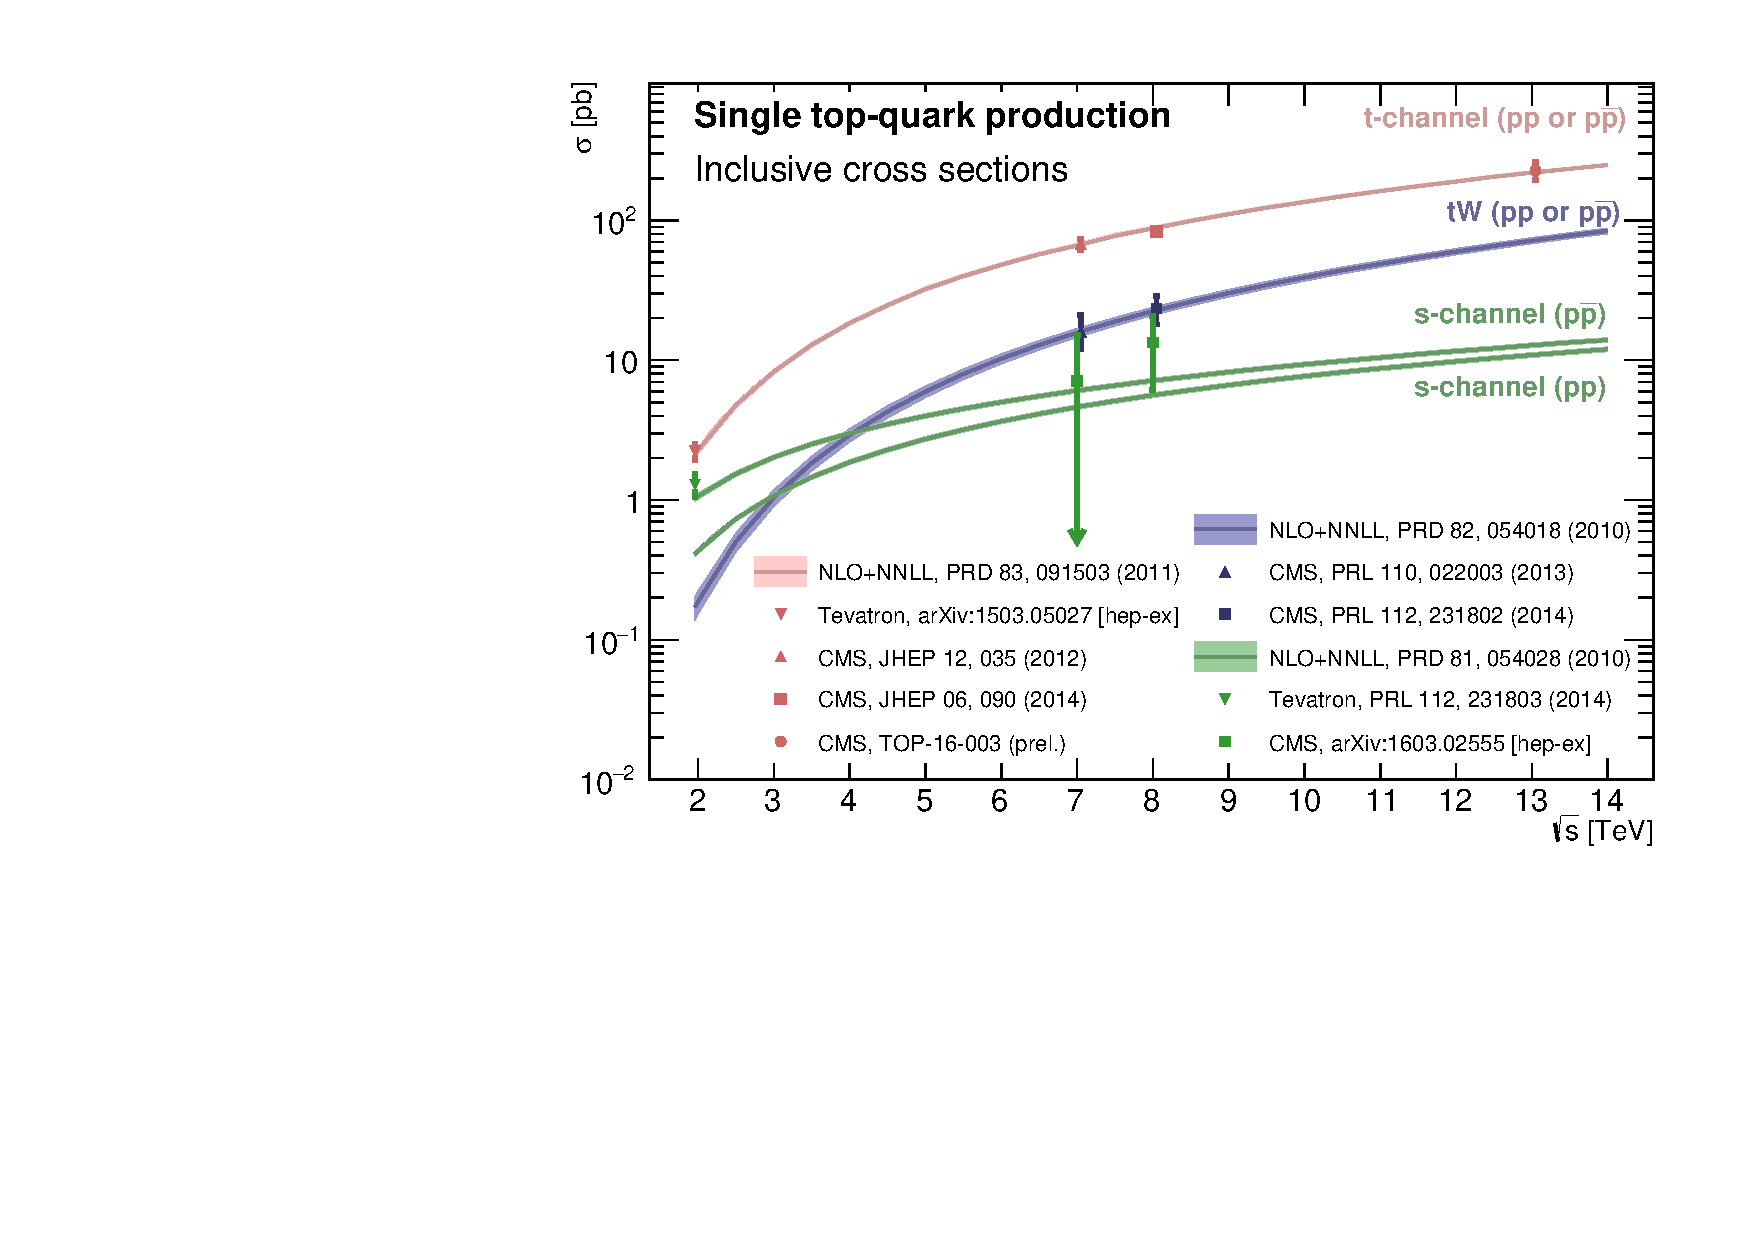
\includegraphics[width=0.7\textwidth]{figures/singletop_sqrts.pdf}
\caption{Overview of single-top-quark cross section measurements for $t$-, tW-, and $s$-channel by the CMS collaboration at various LHC energies.}
\end{center}
\end{figure}

\clearpage

\begin{thebibliography}{99}

\bibitem{CMS-PAS-TOP-16-003}{CMS Collaboration, \emph{Measurement of the inclusive cross section of single top-quark production in the $t$-channel at 13~TeV}, \emph{CMS Physics Analysis} Summary CMS-PAS-TOP-16-003, 2016.}

\bibitem{CMS-PAS-TOP-16-004}{CMS Collaboration, \emph{Measurement of the differential cross section for t-channel single-top-quark production at $\sqrt{\mathrm{s}}=13~\mathrm{TeV}$}, \emph{CMS Physics Analysis Summary} CMS-PAS-TOP-16-004, 2016.}

\bibitem{hathor}{M. Aliev et al., \emph{HATHOR - HAdronic Top and Heavy quarks crOss section calculatoR}, \emph{Comput.Phys.Commun.}~\textbf{182} 1034-1046, 2011.
}

\bibitem{schannel-xsec}{N. Kidonakis, \emph{NNLL threshold resummation for top-pair and single-top production}, \emph{Phys. Part. Nucl.}~\textbf{45} (2014) 714, {\tt arXiv:1210.7813}, 2014.}

\bibitem{CMS-PAS-TOP-13-009}{CMS Collaboration, \emph{Search for $s$ channel single top quark production in pp collisions at $\sqrt{s}$~=~7~and 8~TeV}, submitted to \emph{JHEP}, {\tt arXiv:1603.02555\,[hep-ex]}, 2016.}

\bibitem{wbeyond}{J. A. Aguilar-Saavedra et. al., \emph{W polarisation beyond helicity fractions in top quark decays}, \emph{Nucl.Phys.}~\textbf{B840} 349-378, 2010.}

\bibitem{CMS-PAS-TOP-13-001}{CMS Collaboration, \emph{Measurement of top quark polarisation in t-channel single top quark production}, \emph{JHEP}~\textbf{04} (2016) 073, {\tt arXiv:1511.02138\,[hep-ex]}, 2016.}

\bibitem{fcnc}{S. L. Glashow et. al., \emph{Weak Interactions with Lepton-Hadron Symmetry}, \emph{Phys. Rev.~D}~\textbf{2} 1285, 1970.}

\bibitem{minimal-anom-set}{J. A. Aguilar-Saavedra, \emph{A Minimal set of top anomalous couplings}, \emph{Nucl. Phys.~B}~\textbf{812} 181-204, \texttt{arXiv:0811.3842[hep-ph]}, 2009.}

\bibitem{CMS-PAS-TOP-14-003}{CMS Collaboration, \emph{Search for anomalous single top quark production in association with a photon in pp collisions at $\sqrt{s}=8~\mathrm{TeV}$}, \emph{JHEP}~\textbf{04} (2016) 035, {\tt arXiv:1511.03951\,[hep-ex]}, 2016.}

\end{thebibliography}

\end{document}
